Avant de mener une réflexion sur la définition des normes à adopter pour
des éditions numériques des diagrammes, il est nécessaire de comprendre
dans quel environnement technique, grâce à quels langages et quels
formats elle pourra être implémentée. En effet, dans la chaîne de
traitement d'\eida, si la vectorisation est une fin en soi, elle peut
s'intégrer dans un projet plus ambitieux. La \textit{pipeline} implémentant la
vision artificielle extrait des formats \emph{computable}
(compréhensibles par les machines) constituant une base pour l'édition
scientifique.

\hypertarget{transcription-automatique-des-diagrammes}{%
\subsection{Transcription automatique des
diagrammes}\label{transcription-automatique-des-diagrammes}}

À l'heure actuelle, la transformation des diagrammes en objets
informatiques repose souvent sur l'adaptation d'outils et de pratiques
initialement conçus pour les textes.

Par exemple, l'Académie des Sciences de Berlin-Brandenburg mène depuis
1919 un projet monumental d'édition critique de l'œuvre de Gottfried
Wilhelm Leibniz. Son pendant numérique, Leibniz-Online\footcite{noauthor_leibniz_nodate}, utilise
\LaTeX\xspace comme outil d'édition, tant pour les textes que pour les
diagrammes. La méthode présente certaines limites. Premièrement, \LaTeX\xspace
est un outil dédié au texte ; le tracé des diagrammes aura nécessité
l'adaptation des packages dédiés aux schémas et la création de
nouvelles commandes adaptées aux besoins du projet mais non
standardisées, ce qui limite l'interopérabilité et interroge la
pérennité de ses pratiques de transcription.

Ken Saito (Osaka Prefecture University), spécialiste en histoire des
mathématiques grecques, met au point, au début des années 2010, un outil
informatique nommé DRaFT\footcite{noauthor_draft_nodate} (Fig. \ref{fig:diag_de_young}) pour l'édition des diagrammes présents dans les
manuscrits mathématiques. Cet outil, permettant de poser des points, de
les relier par des segments ou des courbes et d'ajouter des labels,
génère des fichiers \textsc{eps} (format vectoriel) intégrables dans des
documents \LaTeX\xspace.

\citeauthor{reynaud_diagrammes_2017} relève, dans son travail de thèse\footcite[p.292]{reynaud_diagrammes_2017}, les qualités de ce logiciel qui s’adapte relativement bien pour éditer les diagrammes imprimés ou incisés dans des tablettes mathématiques cunéiformes, et permet l'enregistrement de décisions éditoriales\footcite[``Pour chacune des lignes
ainsi définies, il est ensuite possible de choisir selon son statut (présente sur le diagramme,
reconstituée, bordure du document, etc) un style différent (plein, tirets, pointillés, etc).''][p.292]{reynaud_diagrammes_2017}.

Néanmoins, les formats \textsc{tex} et \textsc{eps}, bien adaptés à l'impression,
présentent des limitations en termes de manipulation : les fichiers \textsc{tex}
sont figés une fois compilés, tandis que les fichiers \textsc{eps} nécessitent
des logiciels propriétaires pour être modifiés. De plus, la
transcription manuelle des diagrammes demeure une étape chronophage. Enfin, les deux méthodes présentent des limitations pour rendre compte de toutes les variations infimes de la structure et de l'épaisseur des lignes présentes dans les diagrammes dessinés à la main\footcite[``When a line has a very noticeable thickness, for example, should one choose points on the outer edge of the line, the inner edge, or somewhere in the middle ? When the scribe produces a distinctly rounded vertex to a quadrilateral, should one choose the point of the vertex to be somewhere in the rounded portion of the line or should the editor choose a point outside the line where the two sides would intersect if continued rectilinearly ?''][]{de_young_diagrams_2009}. 

\begin{figure}[H]
          \begin{center}
          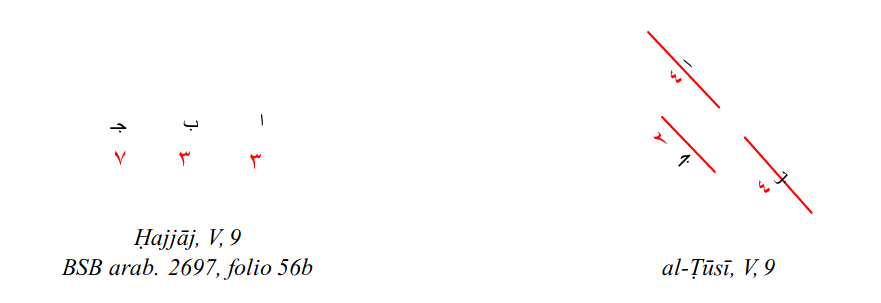
\includegraphics[height=4cm]{figues/diagrammes_de_young.png}
          \end{center}
          \caption{Édition et comparaison de diagrammes des \textit{Éléments} d'Euclide par \citeauthor{de_young_editing_2014}\footcite[p.193]{de_young_diagrams_2009}, utilisant DRaFT.}
          \label{fig:diag_de_young} \end{figure}

\begin{figure}[H]
	\begin{center}
		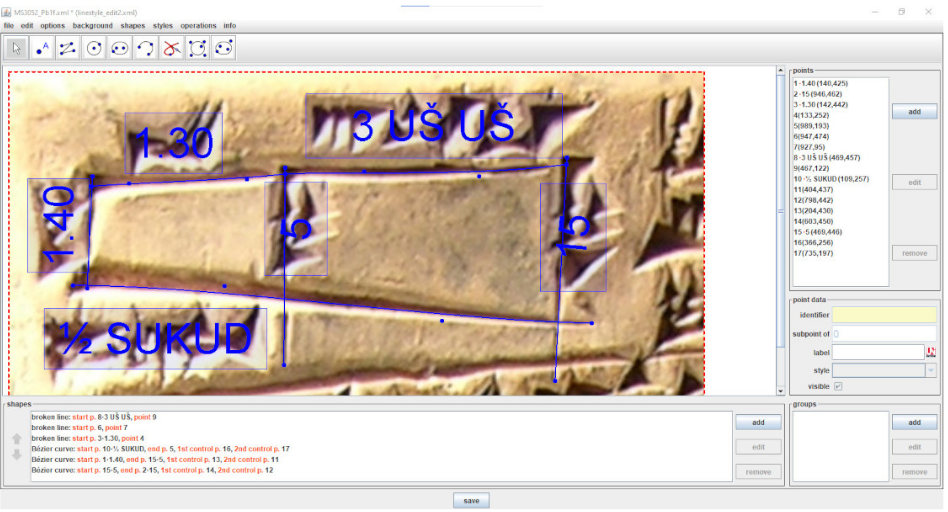
\includegraphics[height=6cm]{figues/diagrammes_de_reynaud.png}
	\end{center}
	\caption{Préparation de l’édition d’un diagramme mathématiques paléo-babyloniens d'une tablette cunéiforme avec le logiciel DRaFT\footcite[Cette capture d'écran est issue du travail de thèse de][p.293]{reynaud_diagrammes_2017}.}
	\label{fig:diag_reynaud} \end{figure}

De manière générale, l'absence de normes pour l'édition numérique des
diagrammes laisse aux projets le choix des outils et méthodes de
transcription, créant un paysage disparate sans pratiques uniformes.
Actuellement, les projets emploient plutôt des outils complets mais
complexes comme GeoGebra ou Inkscape -- logiciels dont la maîtrise
représente un défi pour certains chercheurs -- et procèdent
manuellement.

Pour pallier l'absence de solutions uniformes, l'\ia se présente comme une alternative. Telle qu'implémentée
dans \eida, elle permet d'automatiser génération d'images \svg à partir
d'un large corpus d'images, avec des corrections éventuelles qui restent
beaucoup moins chronophages qu'un tracé manuel de chaque numérisation.
Le \svg est en outre un format léger, interopérable et manipulable.

\hypertarget{idiomes-et-layers-des-formats-computables-et-des-couches-semantiques}{%
\subsection{Idiomes et layers : des formats computables et des
couches
sémantiques}\label{idiomes-et-layers-des-formats-computables-et-des-couches-semantiques}}

\begin{kwote}                            
``One way to understand the structure of a diagram is to break it down
into its component shapes.''\footcite[p.79]{roughan_digital_2014}
                            \end{kwote}  

Dans le fichier \svg (obtenu en sortie du modèle de vectorisation) chaque
objet géométrique est défini avec des éléments
\texttt{\textless{}path/\textgreater{}} et
\texttt{\textless{}circle/\textgreater{}}. La forme encodée dans la
balise correspond à la forme dessinée dans le témoin et la décrit à
l'aide de paramètres mathématiques. Avec ces deux formes fondamentales
il est possible d'encoder et tracer une grande diversité de complexes
géométriques. Par ailleurs le \svg, basé sur le langage \xml, autorise un
balisage des composants individuels en ensembles significatifs (grâce
aux balises \texttt{\textless{}g/\textgreater{}} ou
\texttt{\textless{}symbol/\textgreater{}} notamment)\footcite{noauthor_tutoriel_2024},
lorsqu'il est nécessaire de traiter une série d'unités.

Tout comme \xml est utilisé pour encoder de manière structurée des
données textuelles, ce langage peut être mis au service de
l'enrichissement sémantique de l'élément graphique. Les fichiers \svg peuvent ainsi embarquer des métadonnées. Les balises \xml, en
plus de la description du contenu géométrique, peuvent porter des
attributs tels que des identifiants uniques (\texttt{id}), des
propriétés visuelles (couleur : \texttt{color}, épaisseur de trait :
\texttt{stroke-width})\footcite{noauthor_reference_2024} -- qui
peuvent être extraites automatiquement à partir des images grâce à la
\cv -- et d'autres attributs sémantiques. Ces données
enrichissent considérablement la représentation numérique de l'objet et
ouvrent la voie à des analyses dynamiques et à des visualisations
interactives. En effet, comme le dit Vitali-Rosati, l'édition numérique ne vise plus seulement la production d'un objet ; elle doit assurer un balisage fin des informations qui permette ensuite une exploitation automatique.

\begin{kwote}
``éditer'' ne se réduit plus à mettre en forme pour l'impression et la diffusion sur papier : il s'agit aussi de structurer et de mettre en forme pour le format numérique qui a ses propres particularités. Il ne suffit pas d'essayer de mimer le papier en produisant des versions homothétiques, mais il est nécessaire d'essayer de comprendre comment l'information peut être agencée, structurée et diffusée dans les environnements numériques.''\footcite[p.104]{epron_ledition_2018}
\end{kwote}

Sur un mode \emph{close reading}, il devient possible de développer des
solutions pour isoler, manipuler et transformer les composants
individuels du diagramme. Cela permet de réorganiser, coloriser ou
animer les éléments. En tant qu'objets largement interopérables, les
\svgs peuvent être intégrés dans des pages web, des documents numériques,
et des applications, assurant une accessibilité universelle.

L'encodage en \xml du format \svg permet une interprétation directe par la
machine. Cette caractéristique ouvre la voie à des analyses de grande
échelle, dites de \emph{distant reading}, qui exploitent les capacités
de traitement de corpus de données massifs. En effet, la structure
arborescente et les attributs sémantiques des fichiers \svg servent
d'appui à des algorithmes de fouille de données et de reconnaissance de
similarités. Ces algorithmes peuvent identifier des motifs récurrents,
des structures similaires ; de fait il devient possible de mettre à jour
des relations entre plusieurs diagrammes.

\begin{kwote}                            
``Digital formats, when encoded meaningfully, can be well-suited for
quantitative analyses.''\footcite[p.82]{roughan_digital_2014}
\end{kwote}  

Le contenu géométrique n'est toutefois pas le seul idiome à représenter
dans l'optique d'une édition, et actuellement des discussions sont en
cours concernant l'extraction automatique des labels. Une des
propositions est d'utiliser un format \json, dans un premier temps,
contenant les coordonnées des textes et la direction de lecture. Si les
labels sont transcrits, le contenu sera certainement\footnote{La tâche
  de transcription du texte entourant les diagrammes est un défis
  important en raison de la grande diversité des alphabets, des langues
  et des symboles utilisés, ainsi que de la segmentation spécifique des
  blocs de texte. À l'été 2024, les chercheurs sont encore à la phase de
  préparation des données pour entraîner l'algorithme de segmentation.
 Le format de sortie reste une supposition.} encodé en \xml-\alto,
format qui condense la disposition et la transcription du contenu
textuel. Pour enrichir automatiquement les \svgs avec du texte, des
scripts sont capables d'extraire les coordonnées et le contenu textuel
dans des éléments \svg.

Enfin, l'implémentation de bi-classifications automatiques pourraient
ajouter de l'information globale sur la figure : le caractère
poly/monochromatique et la présence/absence de graduations.

Sur l'extraction de ces idiomes sémantique repose la perspective d'une
recherche de similarité fondée sur des critères explicites : un contenu
géométrique (type de primitives, relations spatiales, position), une
couleur (en se basant sur la valeur des attributs), ou encore le contenu
textuel (transcription et position). La \textit{pipeline} d'\eida vise à
décomposer l'image en une série de représentations qui constituent
autant de calque exploitables et dans lesquels des scripts peuvent
rechercher des similarités. En particulier grâce au \svg, l'information
contenue dans l'image devient éditable, manipulable, enrichie. Grâce à
ce système de calques, les images acquièrent une richesse sémantique,
facilitant des utilisations dans des contextes de fouille, et surtout
d'édition scientifique (Fig.\ref{fig:layers}).

 \begin{figure}[H]
          \begin{center}
          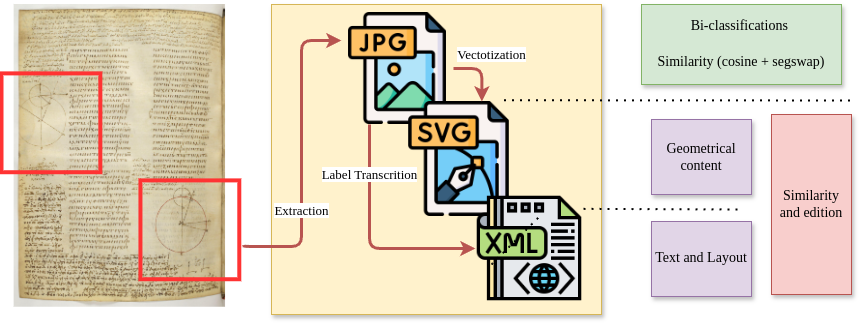
\includegraphics[height=5cm]{figues/layers.png}
          \end{center}
          \caption{Extraction de représentations sémantiquement riches et exploitation. }
          \label{fig:layers} \end{figure}

\hypertarget{une-plateforme-qui-porte-une-methode}{%
\subsection{Une plateforme qui porte une méthode}\label{une-plateforme-qui-porte-une-methode}}

L'intégration de l'\ia dans \aikon ne se limite pas à l'automatisation des
tâches : elle doit s'inscrire dans un environnement de recherche
numérique complet, dédié à l'analyse approfondie de diagrammes
astronomiques. Le constat de l'absence d'outil d'édition dédié à ces
objets justifie l'intégration d'un processus d'édition numérique au sein
d'\aikon. La plateforme et son interface utilisateur ont en effet
l'ambition de favoriser la cohérence des méthodes et leur diffusion au
sein de la communauté scientifique, contribuant ainsi à l'établissement
de pratiques communes pour l'étude des diagrammes astronomiques.

Le modèle de données d'\aikon pourra évoluer pour intégrer les concepts
de \textit{Transcription} et \textit{EditedDiagram}, s'inspirant de la distinction
Témoin/Édition. La \textit{Transcription} représentera la version
informatique d'un diagramme source, reliée à son document d'origine,
tandis que l'\textit{EditedDiagram} correspondra à une nouvelle édition
construite à partir d'une ou plusieurs transcriptions, et reliée à un
chercheur.

 \begin{figure}[H]
          \begin{center}
          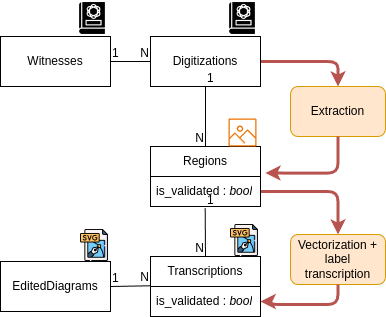
\includegraphics[height=6cm]{figues/modele_edition.png}
          \end{center}
          \caption{Modèle de données hypothétique.}
          \label{fig:modele_edition} \end{figure}

On voit sur la figure \ref{fig:modele_edition} qu'une édition se fond sur une transcription
automatique générée par les modèles de vision. Cette approche, tout en
offrant des avantages en termes d'efficacité, nécessite une intervention
humaine pour corriger les erreurs potentielles des algorithmes,
engendrant ainsi l'existence de multiples versions d'une même
transcription au sein de la plateforme.

La question est importante, car les pistes de correction envisageables divergent selon l'approche adoptée. Une étude fondée sur le \textit{distant reading} d'un corpus volumineux et axée sur la recherche de similitudes ne requiert pas le même niveau d'intervention qu'une analyse fine d'un diagramme dans le cadre d'une édition critique. L'ontologie CIDOC-CRM permet, avec sa notion d'\textit{évènement}, de représenter de modéliser des changements, et de les relier aux objets, aux personnes et éventuellement à un espace-temps associé. En ce sens, il soutiendra certainement les chercheur.ses et les équipes d'ingénieur.es lorsque se posera la question de modéliser des versions des transcriptions.  

En conclusion, la vectorisation occupe une place centrale dans le
projet. Convertissant les images en représentations numériques hautement
structurées, elle permet à la machine de saisir la sémantique de leur
contenu. Le format \svg autorise en outre la manipulation : la correction
ou l'enrichissement par l'ajout de métadonnées et d'attributs
sémantiques dans les balises. Ces propriétés en font le format de base
sur lequel faire reposer une interface d'édition.

Si la vectorisation offre un socle technique solide pour l'édition
numérique, elle ne résout pas pour autant les questions fondamentales
liées à l'interprétation des images, qui relèvent d'une expertise
disciplinaire spécifique.